% Square prism ABCD-A1B1C1D1 with E midpoint of AB1, F midpoint of BC1.
% Diagonals A1C1 (top), AB1, BC1 and bottom diagonal DB drawn; EF dashed.
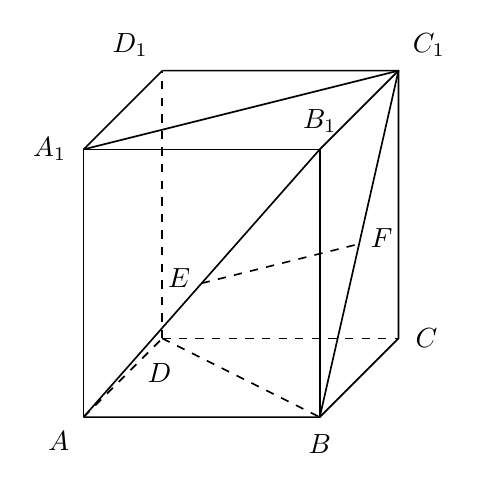
\begin{tikzpicture}[x=1cm,y=1cm,font=\normalsize,
  solidedge/.style={solid,line width=.6pt},
  hidedge/.style={dashed,line width=.6pt},
  ptlabel/.style={font=\normalsize,inner sep=2pt}]
\coordinate (A) at (0,0);
\coordinate (B) at (3,0);
\coordinate (C) at (4,1);
\coordinate (D) at (1,1);
\coordinate (A1) at (0,3.4);
\coordinate (B1) at (3,3.4);
\coordinate (C1) at (4,4.4);
\coordinate (D1) at (1,4.4);
\coordinate (E) at (1.5,1.7);
\coordinate (F) at (3.5,2.2);
% hidden edges
\draw[hidedge] (A)--(D);
\draw[hidedge] (D)--(C);
\draw[hidedge] (D)--(D1);
\draw[hidedge] (D)--(B);
\draw[hidedge] (E)--(F);
% visible cube frame
\draw[solidedge] (A)--(B)--(C)--(C1)--(D1);
\draw[solidedge] (A)--(A1)--(B1)--(B);
\draw[solidedge] (B1)--(C1);
\draw[solidedge] (A1)--(D1);


% face / top diagonals
\draw[solidedge] (A1)--(C1);
\draw[solidedge] (A)--(B1);
\draw[solidedge] (B)--(C1);
% labels kept off the strokes
\node[ptlabel,below left] at ([xshift=-3pt,yshift=-3pt]A) {$A$};
\node[ptlabel,below] at ([yshift=-4pt]B) {$B$};
\node[ptlabel,right] at ([xshift=4pt]C) {$C$};
\node[ptlabel,below,xshift=1pt,yshift=-3pt] at ([xshift=-2pt,yshift=-4pt]D) {$D$};
\node[ptlabel,left] at ([xshift=-4pt]A1) {$A_{1}$};
\node[ptlabel,above] at ([yshift=4pt]B1) {$B_{1}$};
\node[ptlabel,above right] at ([xshift=3pt,yshift=3pt]C1) {$C_{1}$};
\node[ptlabel,above left] at ([xshift=-3pt,yshift=3pt]D1) {$D_{1}$};
\node[ptlabel,left,xshift=3pt,yshift=1pt] at ([xshift=-5pt,yshift=1pt]E) {$E$};
\node[ptlabel,right,xshift=-3pt,yshift=1pt] at ([xshift=5pt,yshift=1pt]F) {$F$};
\end{tikzpicture}
